\documentclass[11pt]{jarticle}

\usepackage[dvipdfmx]{graphicx}

\setlength{\oddsidemargin}{-6.35mm}
\setlength{\textwidth}{171.9mm}

\begin{document}

\title{画像処理実験 第4回}
\author{09430509\\今田将也}
\date{\number\year 年\number\month 月\number\day 日}
\maketitle

\section{cpuで「特徴点らしさ」画像を出力}

資料の例を元に実装を完成させた.

DElem,Elemがimage.hに定義されていなかったので,第3回および第2回を元に移植させた.
そして,Matrix構造体\verb|Matrix *MatrixAlloc|についても移植をおこなった.

最後に,今回の要であるImageFeature関数についてだが,iyに関する計算.そして,iyy,ixxの$\sum$に相当する
計算を行う処理を加えた.以下がその部分のソースコードである.
\begin{verbatim}
    ix = IElem(im, x+u+1, y+v, 1) - IElem(im, x+u-1, y+v, 1);
    iy = IElem(im, x+u, y+v+1, 1) - IElem(im, x+u, y+v-1, 1);
    ixx += ix*ix; // ixx だけでなく ixy,iyy も計算する. 
    iyy += iy*iy;
    ixy += ix*iy;
\end{verbatim}
さらに,DElemには行列
\[
  \left(
    \begin{array}{cc}
      i_{xx} & i_{xy} \\
      i_{xy} & i_{yy} \\
    \end{array}
  \right)
\]
の小さい方の固有値を入れることで求める事ができるが,
2行2列の行列の固有値は2次方程式の解の公式で求めることと同じであるため
解の公式を使った.

\begin{verbatim}
    DElem(im2,x,y) = 
    ((ixx + iyy)+sqrt(pow(ixx+iyy,2.0)-4.0*(ixx*iyy-ixy*ixy)))/2.0;
\end{verbatim}
Wで,自分の周りの上下左右の7マスを見て特徴点を取っている.
この実装で出力された結果は図\ref{out1}に示した.このときのWは7である.
処理時間は3.9GhzのCPUで144msecだった.

\begin{figure}[t]
    \centering
    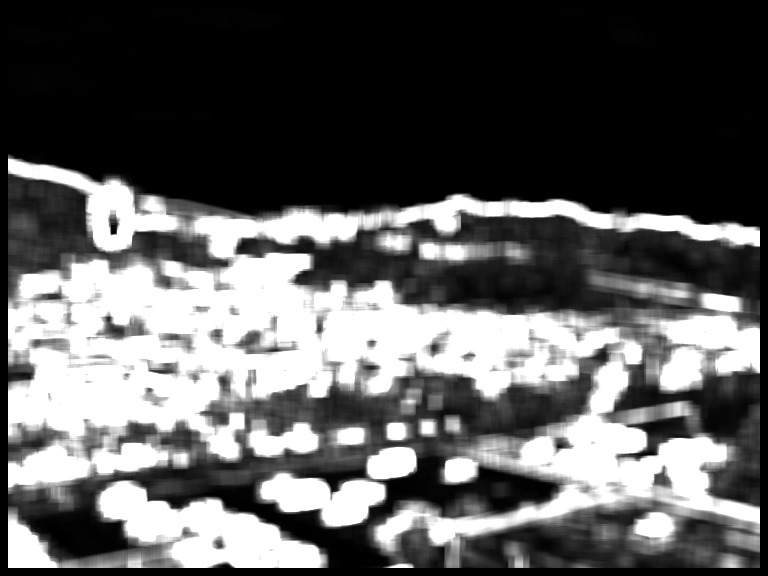
\includegraphics[scale=.5]{out1.jpg}
    \caption{出力結果}
    \label{out1}
\end{figure}

\section{CPUでの分解}
資料を元に,3重ループを2回行うことで実装した.
資料には,
特徴点検出のixx,ixy,iyyは15x15の平滑化であり225個の和である.
これを直接計算するより,横に隣接する15画素の和を中間配列に格納し,
この配列の縦15要素の和によって最終結果を計算するとあるので,それを再現するようにした.
出力結果は図\ref{bunkai}に示す.計算時間は36msecであった.
\begin{verbatim}
        int x,y,u,v,ix,iy;
        for(y=1;y<im->H-1;y++) for(x=W+1;x<im->W-W-1;x++){
              double ixx,ixy,iyy;
              ixx=iyy=ixy=0;
              for(u=-W;u<=W;u++){
                ix = IElem(im, x+u+1, y, 1) - IElem(im, x+u-1, y, 1);
                iy = IElem(im, x+u, y+1, 1) - IElem(im, x+u, y-1, 1);
                ixx += ix*ix;
                iyy += iy*iy;
                ixy += ix*iy;
          }
          DElem(im3,x,y) = ixx;
          DElem(im4,x,y) = ixy;
          DElem(im5,x,y) = iyy;
        }
          for(y=W+1;y<im->H-W-1;y++) for(x=W+1;x<im->W-W-1;x++){
              double ixx,ixy,iyy;
              ixx=iyy=ixy=0;
              for(v=-W;v<=W;v++){
                ixx += DElem(im3, x, y+v);
                ixy += DElem(im4, x, y+v);
                iyy += DElem(im5, x, y+v);
          }
          DElem(im2,x,y) = 
          ((ixx + iyy)+sqrt(pow(ixx+iyy,2.0)-4.0*(ixx*iyy-ixy*ixy)))/2.0;
        }
\end{verbatim}
\begin{figure}[t]
    \centering
    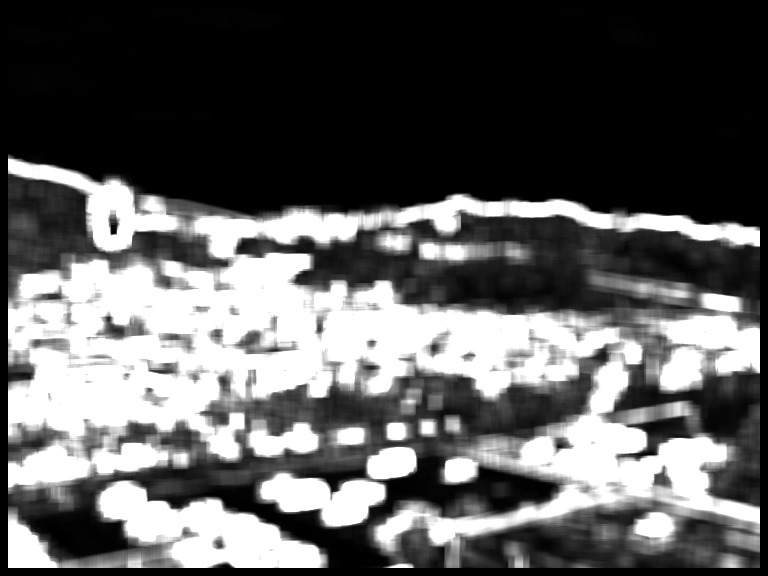
\includegraphics[scale=.5]{out1.jpg}
    \caption{出力結果}
    \label{bunkai}
\end{figure}
\section{実行時間の比較}
CPUとCPU分解の2つの時間を示す.
\begin{table}[h]
    \centering
    \begin{tabular}{l|llll}
    \cline{1-2}
    方法    & 時間(msec) &  &  &  \\ \cline{1-2}
    CPU   & 144      &  &  &  \\
    CPU分解 & 34       &  &  &  \\ \cline{1-2}
    \end{tabular}
    \end{table}

\section{自分で撮影した画像で実験}
作成したCプログラムに,図\ref{mae}を与えて出力された結果を図\ref{out2}に示した.

\begin{figure}[t]
    \begin{minipage}{0.5\hsize}
        \centering
        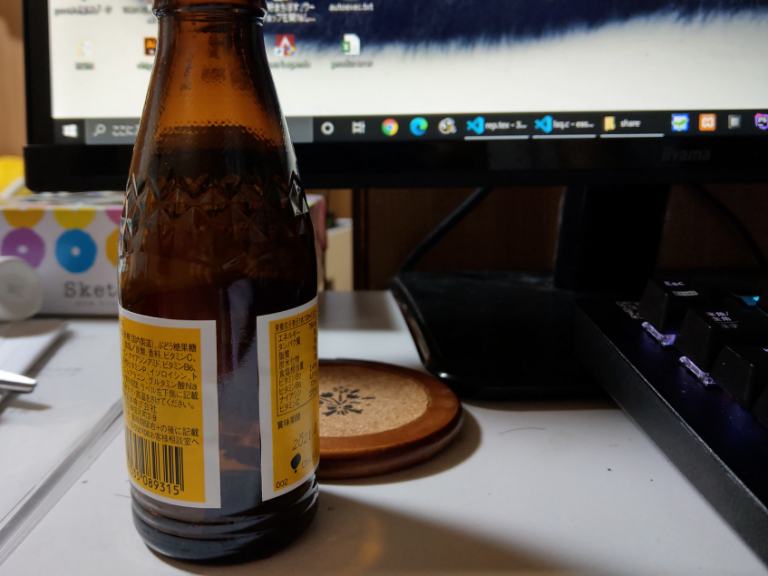
\includegraphics[scale=.3]{mae.jpg}
        \caption{元画像}
        \label{mae}
    \end{minipage}
    \begin{minipage}{0.5\hsize}
        \centering
        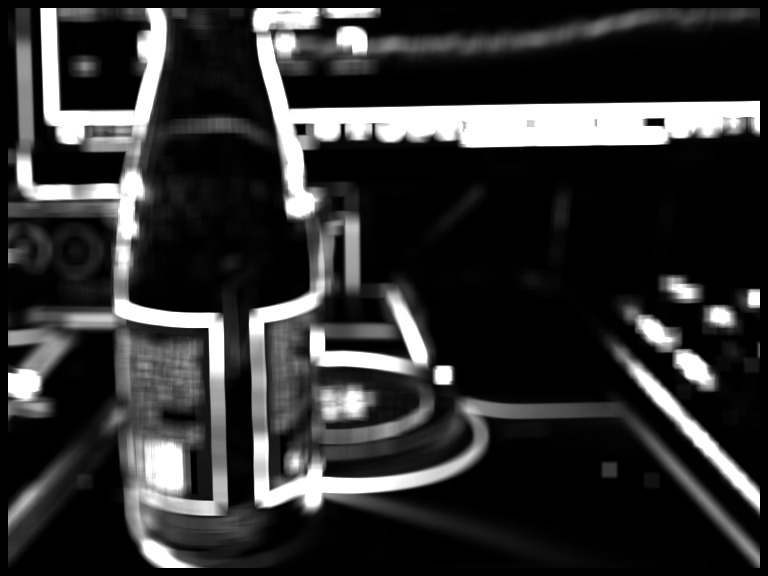
\includegraphics[scale=.3]{out2.jpg}
        \caption{出力結果}
        \label{out2}
    \end{minipage}
\end{figure}

\section{Wの値をコマンドラインから指定}

まず,image.hのImageDrowBoxの宣言にWを整数型で追加した.
そして,使用する際にコマンドライン引数をatoiを使い,整数型に変えることで対応した.
\begin{verbatim}
    ImageDrawBox(im,kk[i][0],kk[i][1],atoi(av[2]));
\end{verbatim}

\section{Wの値を変えて複数回実行}
wの値を0から10まで変えて画像の出力をした.数字が大きくなるにつれて処理時間も増えていった.
図\ref{saisyo}から図\ref{saigo}がその出力結果である.W=2からW=4あたりが綺麗に輪郭が出ている.
W=7以上は輪郭が太くなりすぎてあまり綺麗でなかった.
\begin{figure}[t]
    \begin{minipage}{0.5\hsize}
        \centering
        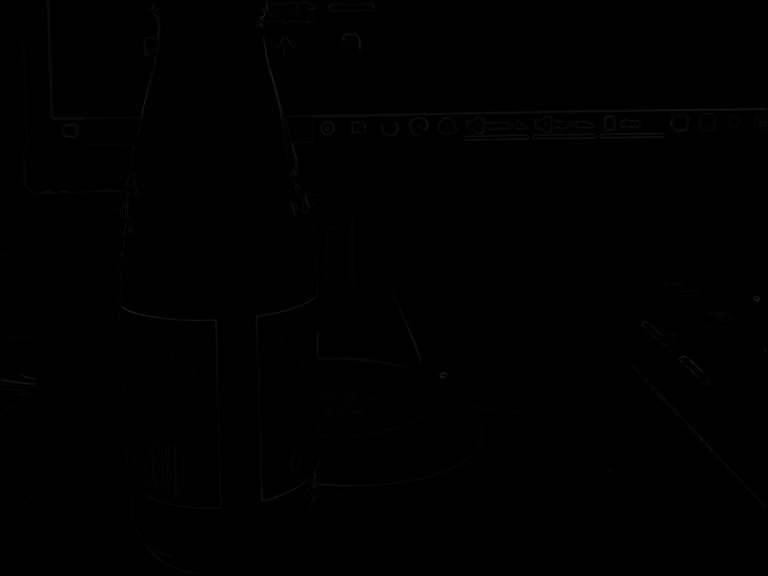
\includegraphics[scale=.3]{w0.jpg}
        \caption{W=0}
        \label{saisyo}
    \end{minipage}
    \begin{minipage}{0.5\hsize}
        \centering
        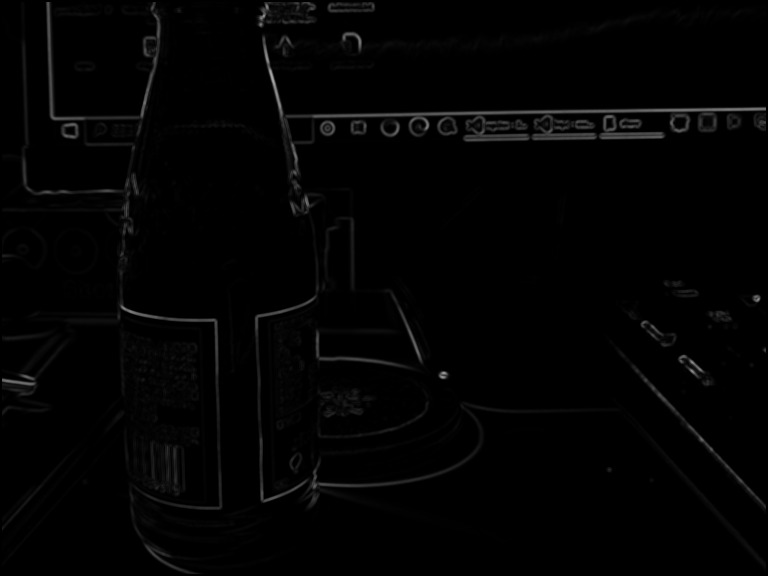
\includegraphics[scale=.3]{w1.jpg}
        \caption{W=1}
    \end{minipage}
\end{figure}
\begin{figure}[t]
    \begin{minipage}{0.5\hsize}
        \centering
        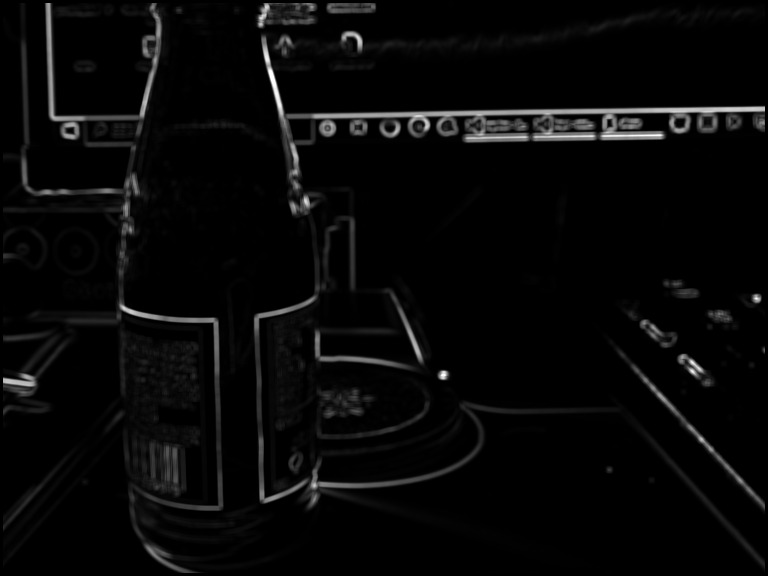
\includegraphics[scale=.3]{w2.jpg}
        \caption{W=2}
    \end{minipage}
    \begin{minipage}{0.5\hsize}
        \centering
        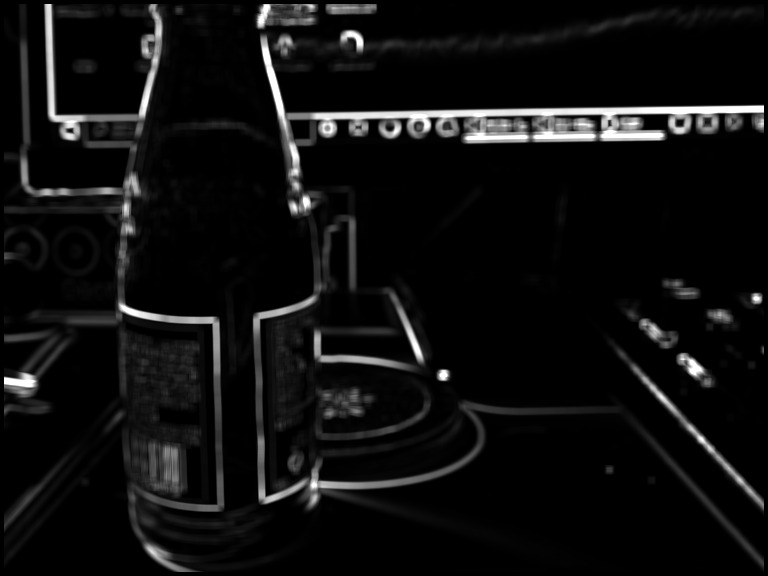
\includegraphics[scale=.3]{w3.jpg}
        \caption{W=3}
    \end{minipage}
\end{figure}
\begin{figure}[t]
    \begin{minipage}{0.5\hsize}
        \centering
        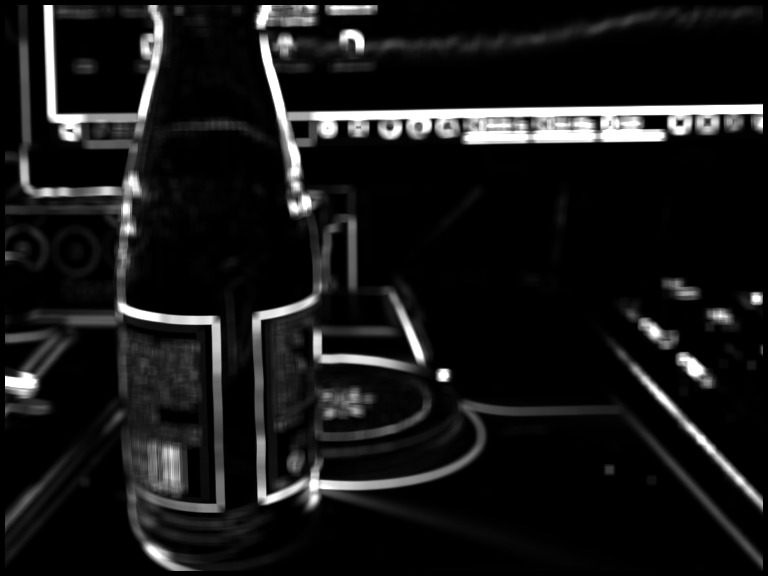
\includegraphics[scale=.3]{w4.jpg}
        \caption{W=4}
    \end{minipage}
    \begin{minipage}{0.5\hsize}
        \centering
        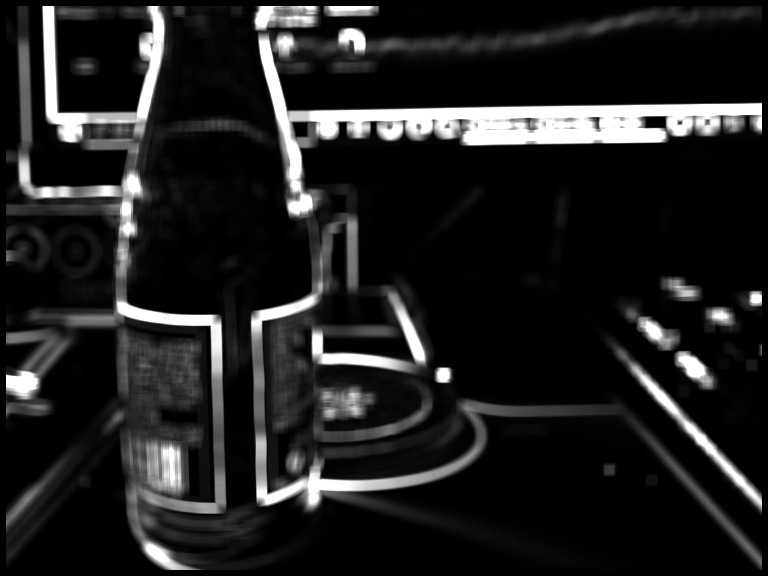
\includegraphics[scale=.3]{w5.jpg}
        \caption{W=5}
    \end{minipage}
\end{figure}
\begin{figure}[t]
    \begin{minipage}{0.5\hsize}
        \centering
        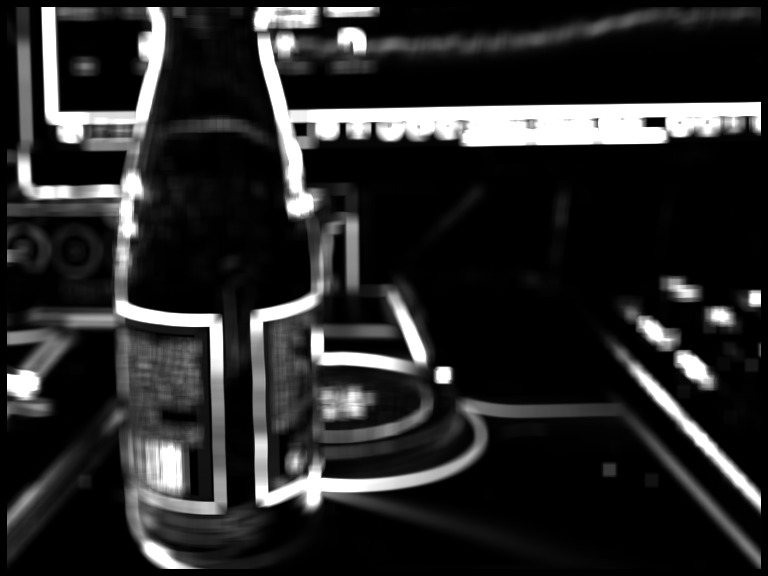
\includegraphics[scale=.3]{w6.jpg}
        \caption{W=6}
    \end{minipage}
    \begin{minipage}{0.5\hsize}
        \centering
        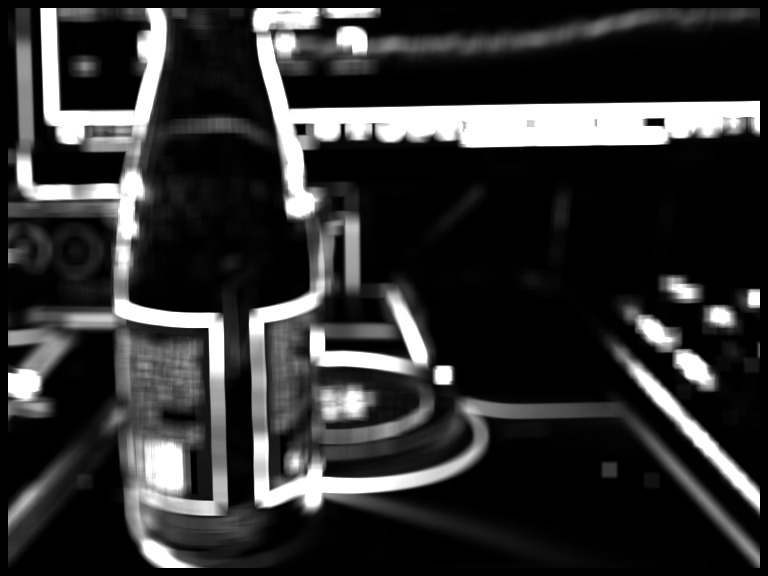
\includegraphics[scale=.3]{w7.jpg}
        \caption{W=7}
    \end{minipage}
\end{figure}
\begin{figure}[t]
    \begin{minipage}{0.5\hsize}
        \centering
        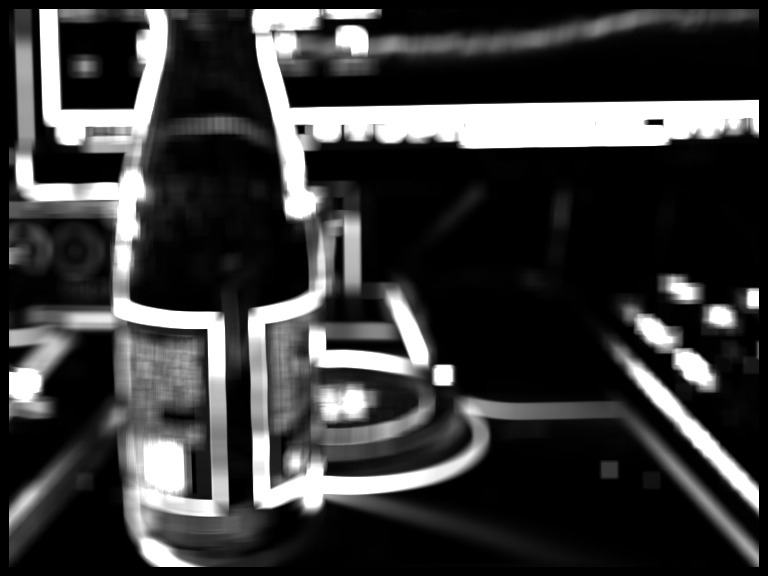
\includegraphics[scale=.3]{w8.jpg}
        \caption{W=8}
    \end{minipage}
    \begin{minipage}{0.5\hsize}
        \centering
        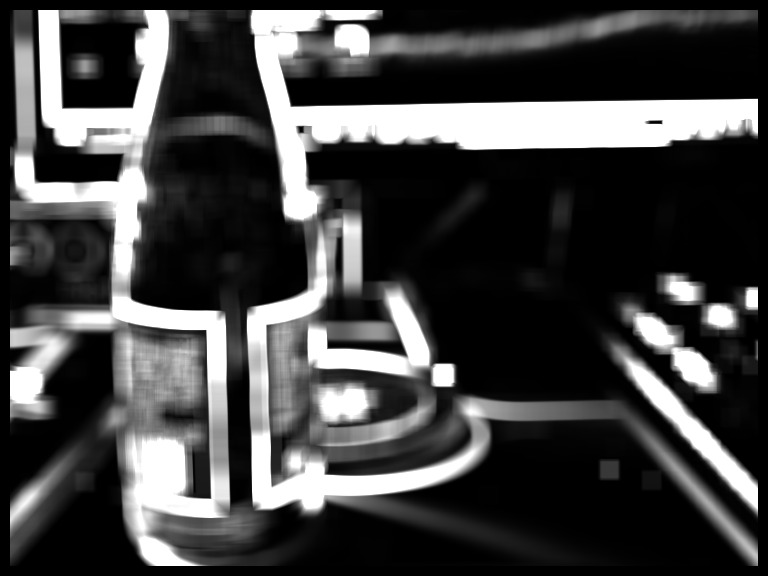
\includegraphics[scale=.3]{w9.jpg}
        \caption{W=9}
    \end{minipage}
\end{figure}
\begin{figure}[t]
    \centering
    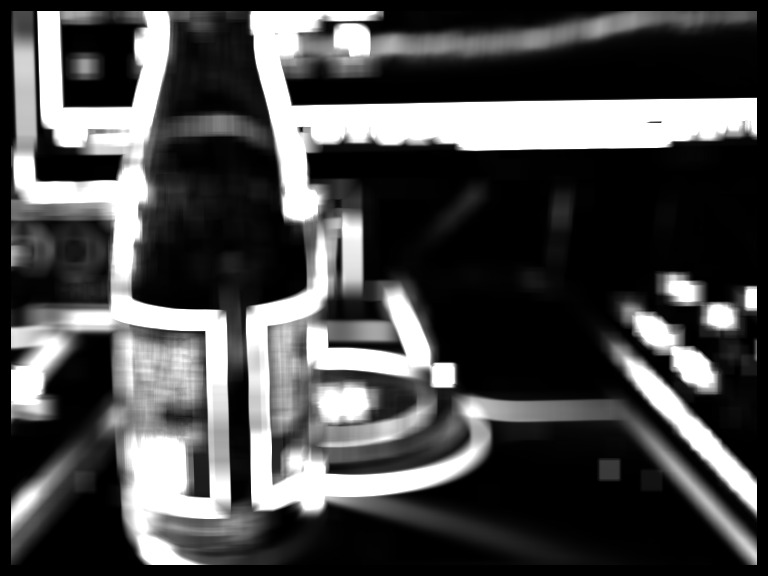
\includegraphics[scale=.5]{w10.jpg}
    \caption{W=10}
    \label{saigo}
\end{figure}

\section{感想}

CPUによる実装を完了させることはでき,Wの値を変えることでどのくらい変化があるのか
ということを画像を並べて比較することができた.
GPUによる実装はできてない上,分解についてもとりあえず実装し,動きまで理解ができていない.

\end{document}
